\chapter{Embedding}\label{chap:embedding}

\section{Graph embedding}\label{sec:embedding:graph_embedding}
    \paragraph{}In this section, we shift our focus towards the creation and embedding of graphs derived from the heap dump data. The process of graph creation involves structuring the data in a way that captures the relationships and connections between the \glspl{structure} and their \glspl{pointer}. Subsequently, we will transform this graphs into low-dimensional vector representations, enabling the application of machine learning techniques to identifying \glspl{structure} containing ssh keys.

    \subsection{Graphs creation}
        \paragraph{}Our graph construction is a meticulously organized process aimed at representing the intricate relationships present within the heap dump data. Comprising three distinct node types - \glspl{structure}, \glspl{pointer}, and \glspl{value_node} - this graph provides a comprehensive view of the data's structure. Our approach commences with the sequential parsing of the heap dump data, enabling the identification of essential \glspl{structure} central to our analytical objectives. These \glspl{structure} form the core nodes of our graph. To establish connections between these \glspl{structure} and their contained data, we further break down each structure into 8-byte blocks. These blocks are then translated into \glspl{value_node} within the graph, serving as connectors bridging the data structures to their specific data. An heuristic approach, grounded in \acrshort{regex}, is employed to identify valid \glspl{pointer} within the heap dump data, with \glspl{pointer} representing a subset of \glspl{value_node}, indicating legitimate \glspl{pointer} references. The scrupulously established connections between \glspl{structure}, \glspl{value_node}, and \glspl{pointer} ensure that the graph accurately mirrors the intricate relationships found within the heap dump data. This comprehensive graph construction process is efficiently implemented in Rust, making effective use of the Petgraph library to handle the complexities of heap dump data and graph representation, offering superior efficiency compared to a Python-based implementation.

        \paragraph{}In the following image \ref{fig:graph_embedding:graph_creation_process}, we can see the \glspl{structure} nodes representing in blue, containing \glspl{pointer} nodes in orange and \glspl{value_node} nodes in gray. 

        \begin{figure}[H]
            \centering
            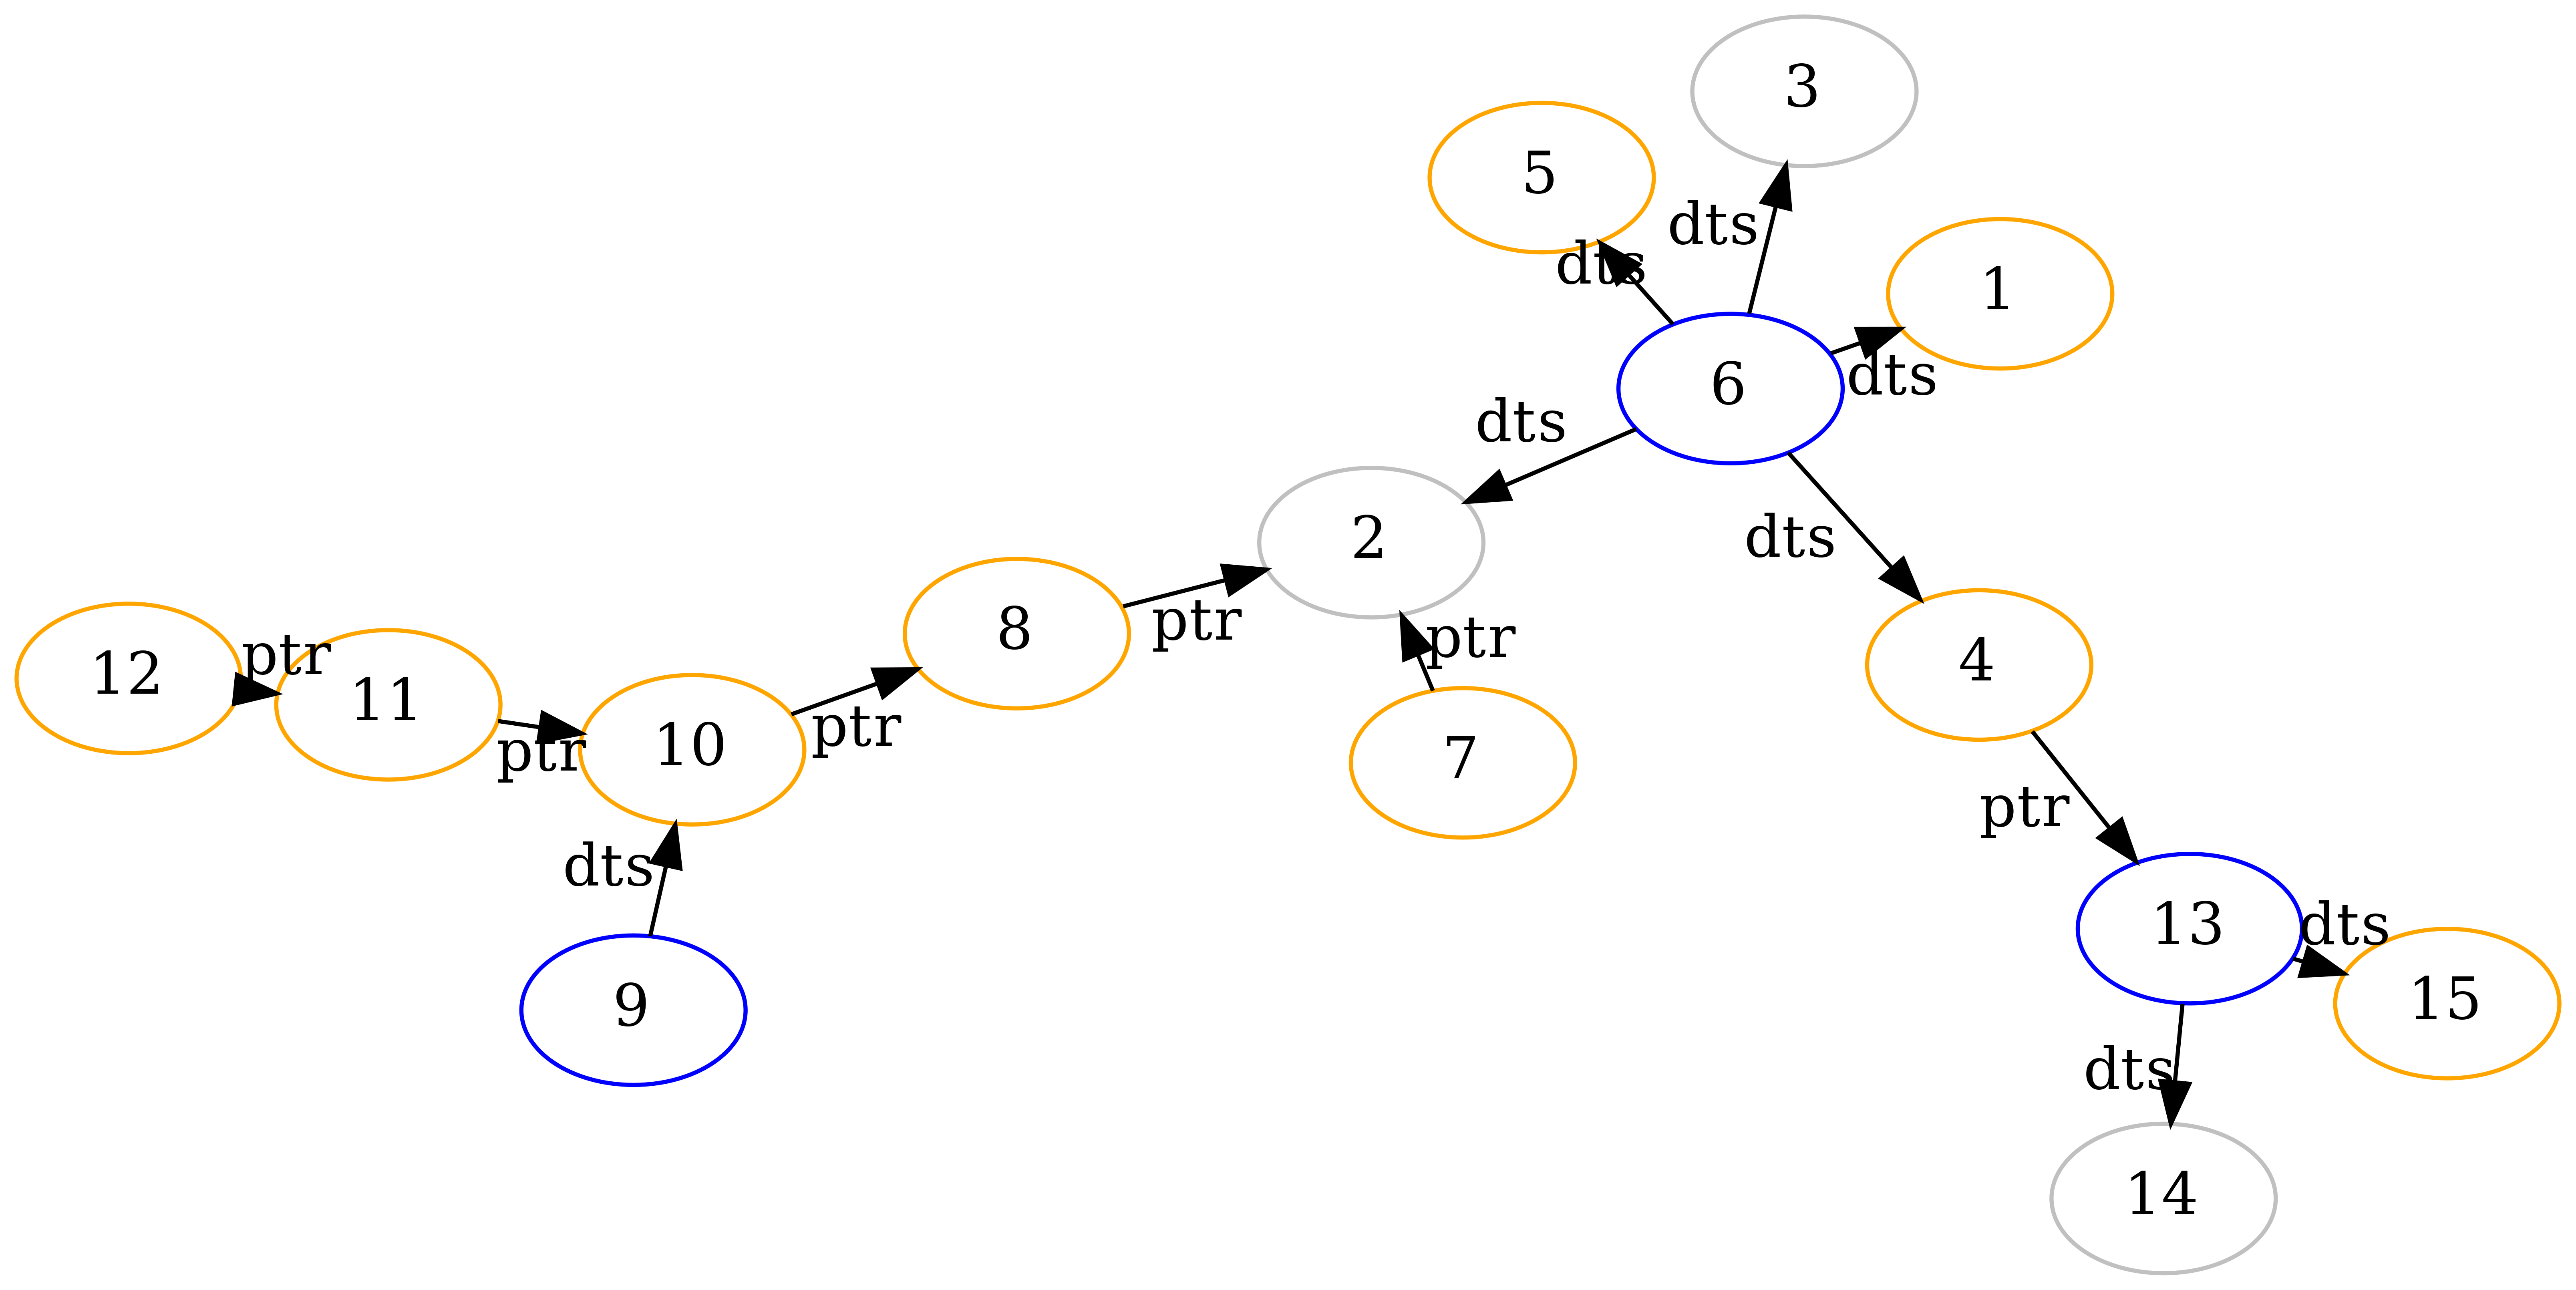
\includegraphics[width=0.9\textwidth]{img/graph_embeding/graph_explain.png}
            \caption{Graph creation process}
            \label{fig:graph_embedding:graph_creation_process}
        \end{figure}

        \paragraph{}After the construction of the graph, we can use graphviz (and the DOT language)\cite{farin_graphviz_2004} to visualize the graph, using the command :
        \begin{lstlisting}[language=bash]
            sfdp -Gsize=67! -Goverlap=prism -Tpng dot_file > image.png
        \end{lstlisting}

        \paragraph{}The following image is an example of the creation of the graph from the file \path{./Training/Training/scp/V_7_8_P1/16/302-1644391327-heap.raw} without \glspl{value_node} to enhance clarity.
        \begin{figure}[H]
            \centering
            \includegraphics[width=0.9\textwidth]{img/graph_embeding/test_graph_from_302-1644391327_no_vn-sfdp.png}
            \caption{Graph example}
            \label{fig:graph_embedding:graph_example}
        \end{figure}

    \subsection{Graphs embedding}

    \begin{algorithm}
        \caption{Sorting Algorithm (e.g., Bubble Sort)}
        \begin{algorithmic}
            \State \textbf{INPUT} arr[] \Comment{An array to be sorted}
            \State $n \gets$ length of arr[]
            \For{$i \gets 0$ \textbf{to} $n-1$}
                \For{$j \gets 0$ \textbf{to} $n-i-1$}
                    \If{arr[$j$] $>$ arr[$j+1$]}
                        \State swap(arr[$j$], arr[$j+1$]) \Comment{Swap elements if out of order}
                    \EndIf
                \EndFor
            \EndFor
            \State \textbf{OUTPUT} arr[] \Comment{Sorted array}
        \end{algorithmic}
     \end{algorithm}